\documentclass{beamer}

\usepackage{beamerthemesplit}
\usepackage{verbatim}
\usepackage[normalem]{ulem}

\usepackage{xcolor}

\usepackage{hyperref}

\definecolor{gold}{rgb}{1.,0.84,0.}
\definecolor{brightred}{rgb}{1.,0.4,0.4}
\definecolor{mygray}{RGB}{200,200,200}
\definecolor{lightsteelblue}{RGB}{176,196,222}
\definecolor{lightskyblue}{RGB}{135,206,250}
\definecolor{cadetblue}{RGB}{95,158,160}

\usetheme{default}
\usecolortheme{mule}

\usefonttheme{serif}

%\DeclareGraphicsExtensions{.pdf,.png,.jpg}

\newcommand{\snr}{$S/N$}
\newcommand{\snT}{$(S/N)_{\textrm{size}}$}
%\newcommand{\snT}{$\left( \frac{S}{N}\right)_{\textrm{size}}$}
\newcommand{\snflux}{$(S/N)_{\textrm{flux}}$}
%\newcommand{\snflux}{$\left( \frac{S}{N}\right)_{\textrm{flux}}$}

\newcommand{\lensfit}{\texttt{LENSFIT}}
\newcommand{\numba}{\texttt{Numba}}
\newcommand{\python}{\texttt{Python}}
\newcommand{\ngmix}{\texttt{ngmix}}
\newcommand{\shear}{{\bf g}}
\newcommand{\redmapper}{redMaPPer}
\newcommand{\est}{$e$}
\newcommand{\mest}{e}

\newcommand{\mcalR}{$R$}
\newcommand{\mcalRpsf}{$R^{p}$}
\newcommand{\mcalRS}{$R_{S}$}

\newcommand{\prelim}{{\bf{\it Preliminary}}}



\title{Update on Metacalibration for Weak Lensing Shear Measurement}
\author{Erin Sheldon}
\institute{Brookhaven National Laboratory}

% http://texblog.net/latex-archive/plaintex/beamer-footline-frame-number/
% to add the page (frame ) number and not screw up the bottom line
% works for split themes?
\expandafter\def\expandafter\insertshorttitle\expandafter{%
      \insertshorttitle\hfill%
        \insertframenumber\,/\,\inserttotalframenumber}

% suppress navigation bar
\beamertemplatenavigationsymbolsempty
\setbeamertemplate{footline}{}

\begin{document}

\frame{\titlepage}


\setbeamertemplate{background canvas}[vertical shading][bottom=mgray,top=mblack]

\frame
{
    \frametitle{Outline}

    \setbeamerfont*{itemize/enumerate body}{size=\Large}
    \setbeamerfont*{itemize/enumerate subbody}{parent=itemize/enumerate body}
    \setbeamerfont*{itemize/enumerate subsubbody}{parent=itemize/enumerate body}
 
    \begin{itemize}

        \item Metacalibration Reminder

        \item Selection Effects

        \item Metacal on Y3

    \end{itemize}

}

\frame
{
    \frametitle{Shear Accuracy Requirements}

    \setbeamerfont*{itemize/enumerate body}{size=\Large}
    \setbeamerfont*{itemize/enumerate subbody}{parent=itemize/enumerate body}
    \setbeamerfont*{itemize/enumerate subsubbody}{parent=itemize/enumerate body}
 
    \begin{itemize}

        \item In order to measure the Dark Energy equation of state
            to the desired accuracy for DES/LSST, we must measure
            shear with exquisite accuracy.

            {\color{lightskyblue}
                \begin{equation}
                    \gamma = (1 + m ) \times \gamma_{true} + c \nonumber
                \end{equation}
            } 

        \item LSST Requirements
            \begin{itemize}
                \item Multiplicative errors: {\color{gold} $m \lesssim 0.001$}
                \item Additive errors: {\color{brightred} $c \lesssim 0.0001$}
            \end{itemize}


    \end{itemize}

}



\frame
{
    \frametitle{Metacalibration Idea from Eric Huff}

    \setbeamerfont*{itemize/enumerate body}{size=\normalsize}
    \setbeamerfont*{itemize/enumerate subbody}{parent=itemize/enumerate body}
    \setbeamerfont*{itemize/enumerate subsubbody}{parent=itemize/enumerate body}
 
    \begin{itemize}

        \item Say we have a biased shear estimator {\color{gold} $e$}.  Then we can write
            {\color{gold}
                \begin{align} \label{eq:Eexpand}
                    \mest(\gamma) &= \mest|_{\gamma=0} + \gamma ~ \frac{ \partial \mest }{ \partial \gamma }\bigg|_{\gamma=0}  + ... \nonumber \\
                                  &\approx \gamma R \nonumber
                \end{align}
            } 
        \item Use image manipulation to estimate the derivative of the
            estimator with respect to shear
            {\color{gold}
                \begin{equation}
                    R = \frac{\mest(+\Delta\gamma) - \mest(-\Delta\gamma)}{2 \Delta \gamma} \nonumber 
                \end{equation}
            }
            \begin{itemize}
                \item Deconvolve the PSF
                \item Shear the image by a small amount
                \item Reconvolve by the PSF.  Use a slightly larger PSF to suppress
                    the noise amplification
                \item Add noise field to cancel correlated noise
            \end{itemize}


    \end{itemize}

}



\frame
{
    \frametitle{Selection Effects}

    \setbeamerfont*{itemize/enumerate body}{size=\Large}
    \setbeamerfont*{itemize/enumerate subbody}{parent=itemize/enumerate body}
    \setbeamerfont*{itemize/enumerate subsubbody}{parent=itemize/enumerate body}
 

    \begin{itemize}

        \item  Applying a selection to objects, for example on the signal-to-noise
            ratio \snr, can indirectly select the shapes of galaxies and result
            in a biased shear recover.

        \item For example, putting a threshold on \snr\ tends to select less
            elliptical galaxies.

    \end{itemize}

}

\frame
{
    \frametitle{Selection Effects}

    \setbeamerfont*{itemize/enumerate body}{size=\large}
    \setbeamerfont*{itemize/enumerate subbody}{parent=itemize/enumerate body}
    \setbeamerfont*{itemize/enumerate subsubbody}{parent=itemize/enumerate body}
 
    \begin{itemize}

        \item If we have a selection function $S$ that has some dependence
            on elliticity, then the mean ellipticity
            can be biased

            \begin{align}
                {\color{gold} \langle \mest S \rangle = \int S(\mest)~P(\mest)~\mest~d\mest},
            \end{align}


        \item We can use the same quantities we have already calculated
            to correct for selections. 

            \begin{align}
                \frac{\partial \langle \mest \rangle}{\partial \gamma}\bigg|_{\gamma=0} &\approx
                \langle R \rangle + \frac{\langle \mest S^+ \rangle - \langle \mest S^- \rangle}{2 \Delta \gamma} \nonumber \\
                &\equiv {\color{gold} \langle R \rangle + \langle \mbox{\mcalRS} \rangle},
            \end{align}

            Where $\langle e S^+ \rangle$ represents the mean unsheared shape, with selection
            applied to the positively sheared parameters.  Similar for $\langle e S^- \rangle$.

    \end{itemize}

}

\frame
{
    \frametitle{Catalog Fields described on the wiki}


    {\small
    \href{https://cdcvs.fnal.gov/redmine/projects/deswlwg/wiki/Matched\_catalogs}{https://cdcvs.fnal.gov/redmine/projects/deswlwg/wiki/Matched\_catalogs}
    }

    For example
    \begin{itemize}
        \item {\color{gold} {\texttt mcal\_s2n\_r}} is the unsheared \snr\
        \item {\color{gold} {\texttt mcal\_s2n\_r\_1p}} sheared by $g_1  = +0.01$
        \item {\color{gold} {\texttt mcal\_s2n\_r\_1m}} sheared by $g_1  = -0.01$
        \item {\color{gold} {\texttt mcal\_s2n\_r\_2p}} sheared by $g_2  = +0.01$
        \item {\color{gold} {\texttt mcal\_s2n\_r\_2m}} sheared by $g_2  = -0.01$
    \end{itemize}
}

\frame
{

    \frametitle{Simulation}

    \begin{itemize}
        \item PSF Moffat $e=0.05, r_{50} = 0.9$ arcsec.
        \item Flux/size from COSMOS 25.2 sample
        \item $S/N$ down to 2.
        \item Bulge+Disk with knots of star formation
        \item Apply threshold of $5-\sigma$ {\em before} metacal, so this
            mimics thresholds in DESDM that we cannot correct for.
    \end{itemize}


}

\frame
{
    \frametitle{\snr}
 
    \begin{center}
        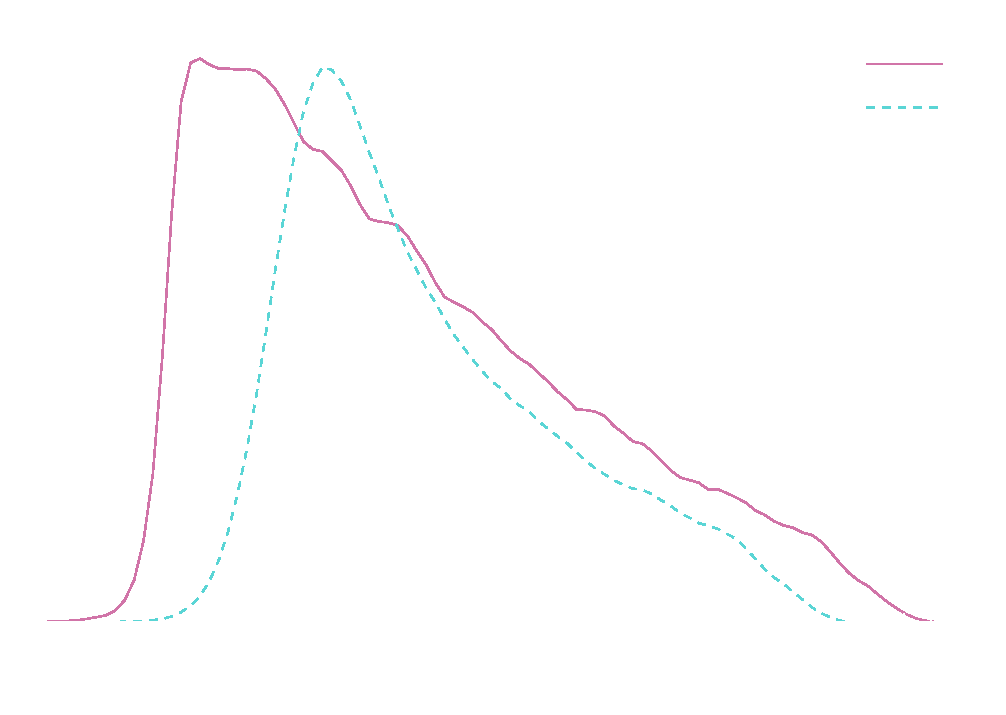
\includegraphics[width=\textwidth]{run-bdj03mcal01-s2n-inv.pdf}
        \newline
    \end{center}



}

\frame
{
    \frametitle{$r_{50}$}
 
    \begin{center}
        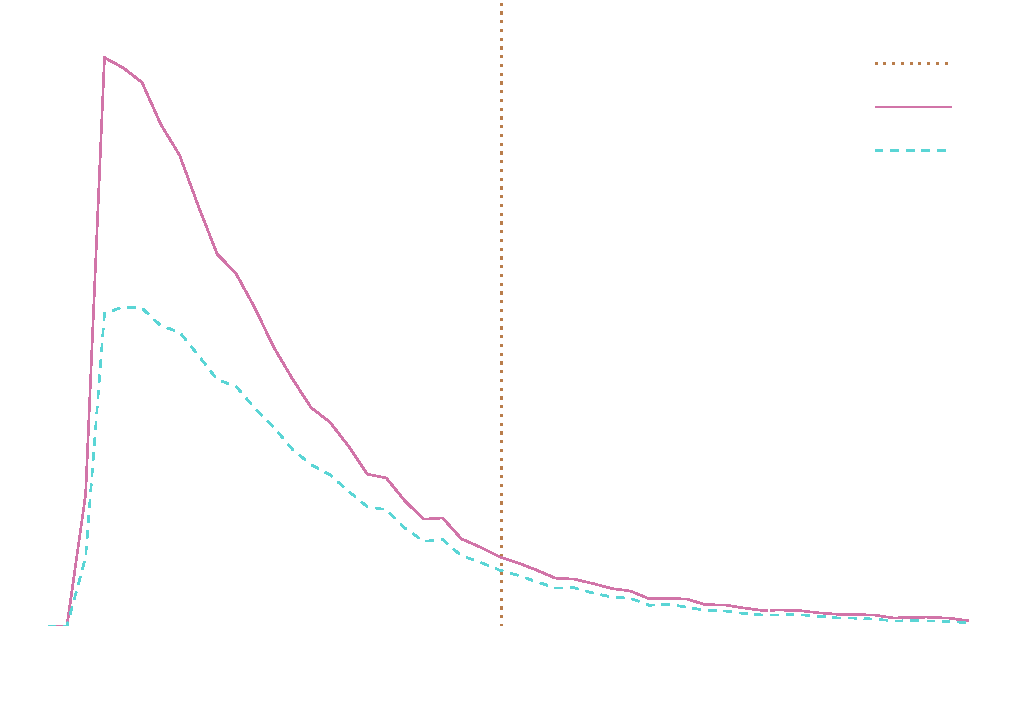
\includegraphics[width=\textwidth]{run-bdj03mcal01-r50-inv.pdf}
        \newline
    \end{center}



}



\frame
{
    \frametitle{\snr\ Cuts}
 

    \begin{columns}
        \begin{column}{0.4\textwidth}
            \begin{itemize}
                \item Select objects with \snr\ greater than some threshold.
            \end{itemize}
        \end{column}
        \begin{column}{0.6\textwidth}
            \begin{center}
            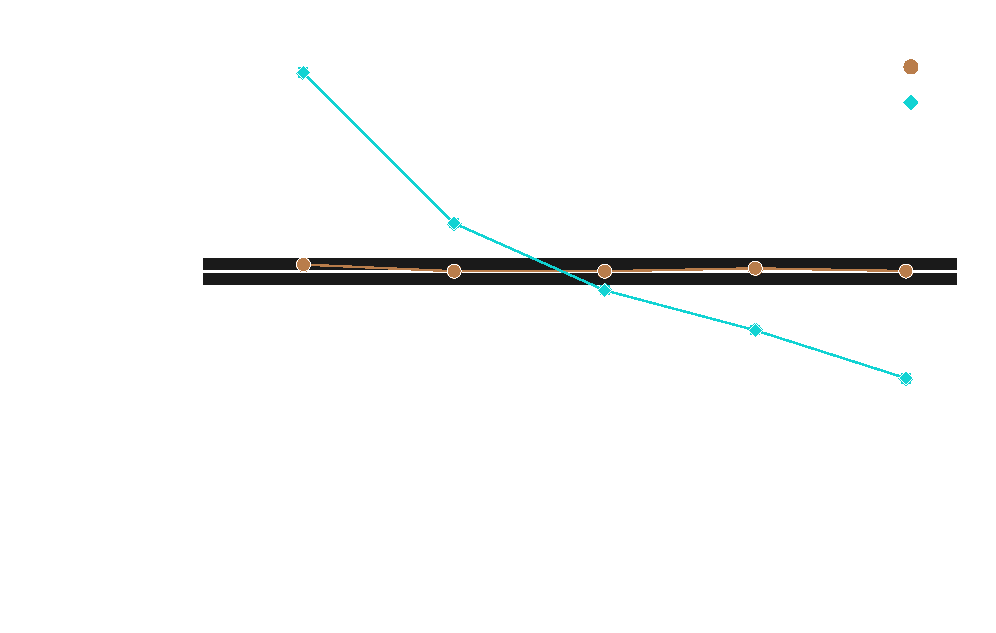
\includegraphics[width=\textwidth]{mc-select-bias-thresh-with-nocorr-inv.pdf}
                \newline
            \end{center}
        \end{column}
    \end{columns}


}

\frame
{
    \frametitle{\snr\ Cuts}
 

    \begin{columns}
        \begin{column}{0.4\textwidth}
            \begin{itemize}
                \item Select objects with \snr\ greater than some threshold.
            \end{itemize}
        \end{column}
        \begin{column}{0.6\textwidth}
            \begin{center}
            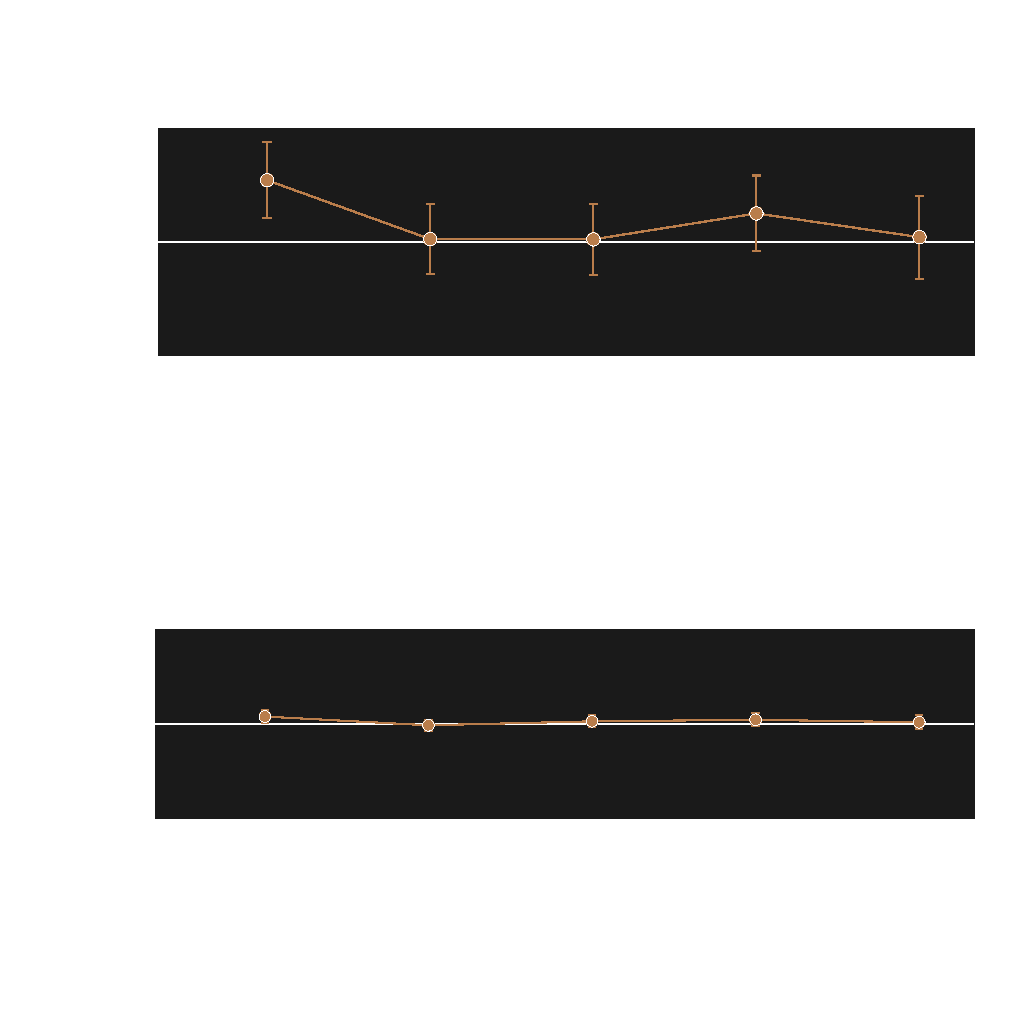
\includegraphics[width=\textwidth]{mc-select-bias-thresh-inv.pdf}
                \newline
            \end{center}
        \end{column}
    \end{columns}


}



\frame
{
    \frametitle{Metacal on Y3}

    \setbeamerfont*{itemize/enumerate body}{size=\Large}
    \setbeamerfont*{itemize/enumerate subbody}{parent=itemize/enumerate body}
    \setbeamerfont*{itemize/enumerate subsubbody}{parent=itemize/enumerate body}
 
    \begin{itemize}

        \item Tested $r,i,z$ on 1000 tiles.

        \item DESDM psf

        \item The null tests might look a bit better than Y1 psf V2
            

    \end{itemize}

}

\frame
{
    \frametitle{PSF ``Leakage''}
 
   Cut to $S/N > 10~~ \&\&~~ T > 0.5 T_{PSF}$
   \newline
   Error on slope $\sim 0.005$


    \begin{center}
    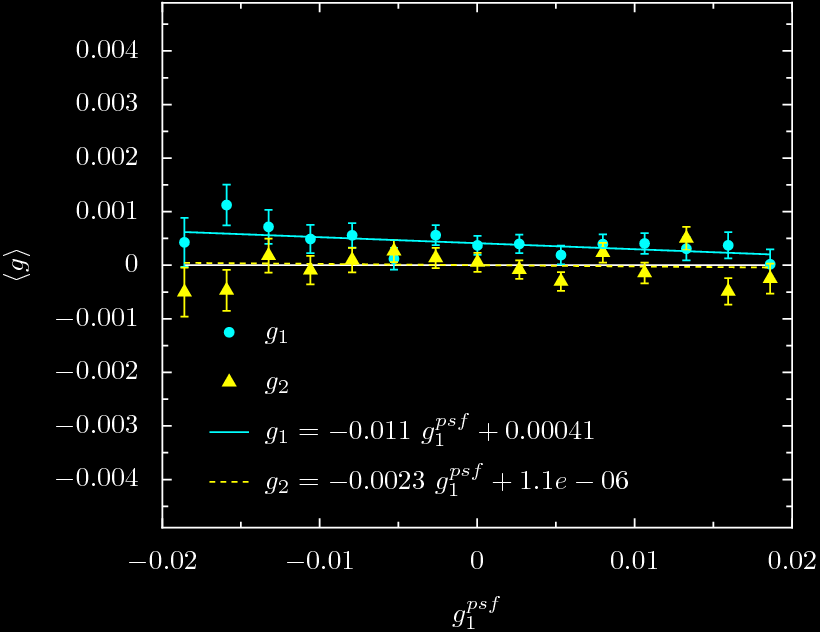
\includegraphics[width=0.8\textwidth]{y3-ThalfTpsf-g1psf-inv.png}
    \end{center}


}

\frame
{
    \frametitle{PSF ``Leakage''}
 
   Cut to $S/N > 10 ~~ \&\& ~~ T > 0.5 T_{PSF}$
   \newline
   Error on slope $\sim 0.005$


    \begin{center}
    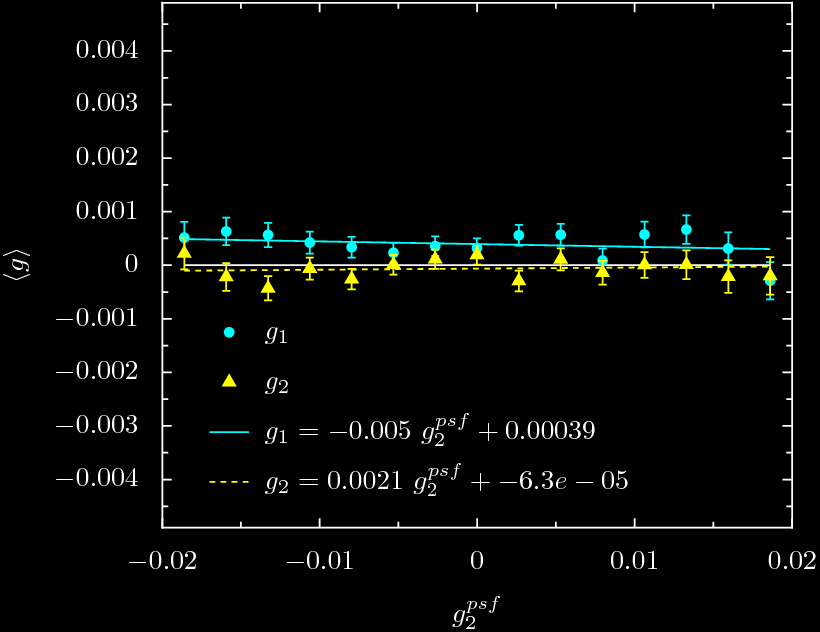
\includegraphics[width=0.8\textwidth]{y3-ThalfTpsf-g2psf-inv.png}
    \end{center}


}




\end{document}
